\section{Sensitivitätsanalyse}{
	Um den Einfluss von Alpha und Beta zu verdeutlichen, folgt ein Beispiel bezogen auf die Situation einer Ameisenkolonie. In Abbildung \ref{parameter_start} zu sehen ist eine Ameisenkolonie, die neu aufgebaut wurde. Diese Kolonie hat Zugang zu zwei Nahrungsquellen: Einer Wasserquelle und einer Zuckerwasserquelle. Für die Ameisen deutlich wertvoller ist die Zuckerwasserquelle, allerdings ist diese auch weiter entfernt. Zu sehen sind auch bereits Ameisen, die auf die Nahrungssuche gehen. Hierbei ist zu beachten, dass die Ameisen im derzeitigen Zustand gleich verteilt sind.
	\begin{figure}[h]
		\centering
		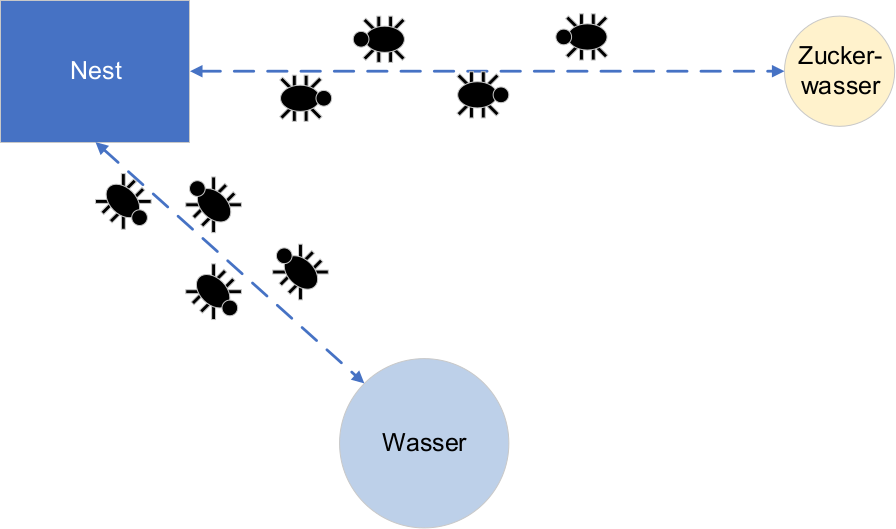
\includegraphics[width=0.9\linewidth]{images/AntAlgorithm_start.png}
		\caption{Modellierung einer Ameisenkolonie mit zwei unterschiedlichen Nahrungsquellen.}
		\label{parameter_start}
	\end{figure}
	Je länger die Nahrungssuche abläuft, desto höher wird der Pheromonwert der Strecke, an deren Ende das Zuckerwasser zu finden ist. In der im vorherigen Kapitel vorgestellten Formel sind Alpha und Beta die beiden Parameter, über die bestimmt wird wie sehr der Pheromonwert gewichtet wird. 
	
	Die folgenden Beispiele basieren auf der Annahme, dass genügend Zeit vergangen ist, damit die Ameisenkolonie die Strecken ausreichend mit Pheromonen belegen konnte.
	Zusätzlich zu beachten ist, dass Alpha und Beta laut Definition der vorliegenden Architektur gemeinsam $1$ ergeben müssen.
	
	\subsection{$\alpha$ hoch - $\beta$ niedrig}
	Wird Alpha maßgeblich größer gewählt als Beta, so wird der Pheromonwert der Strecke höher gewichtet als die Länge. Auf das Beispiel angewendet bedeutet das, dass die Ameisen - wie in Abbildung \ref{parameter_a>b} - deutlich wahrscheinlicher das Zuckerwasser einsammeln. Diese Situation entspricht der Realität und ist die logischste. Denn der Pheromonwert soll ein Leitwert für die restliche Kolonie sein, welche Strecke wertvoll ist.
	\begin{figure}[h]
		\centering
		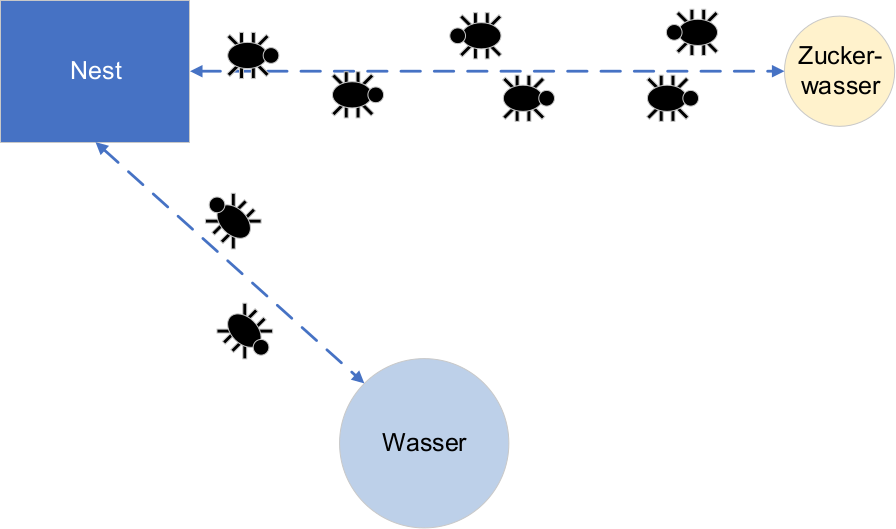
\includegraphics[width=0.7\linewidth]{images/AntAlgorithm_alphaMbeta.png}
		\caption{Modellierung der Parametereinstellung, sodass der Wert Alpha merklich größer als der von Beta ist.}
		\label{parameter_a>b}
	\end{figure}
	
	\subsection{$\alpha$ mittel - $\beta$ mittel}
	Ein Fall, der ebenso möglich ist und in einem gewissen Rahmen Sinn ergibt, ist dass die beiden Parameter Alpha und Beta gleich groß gewählt werden. Hierbei würde sich das in Abbildung \ref{parameter_a=b} ergeben. Im Gegensatz zu Abbildung \ref{parameter_a>b} ist zu erkennen, dass mehr Ameisen den kürzeren Weg zur Wasserquelle wählen. Dies liegt daran, dass der Weg dorthin kürzer ist, was durch die neue Parameterverteilung höher gewichtet wird.
	\begin{figure}[h]
		\centering
		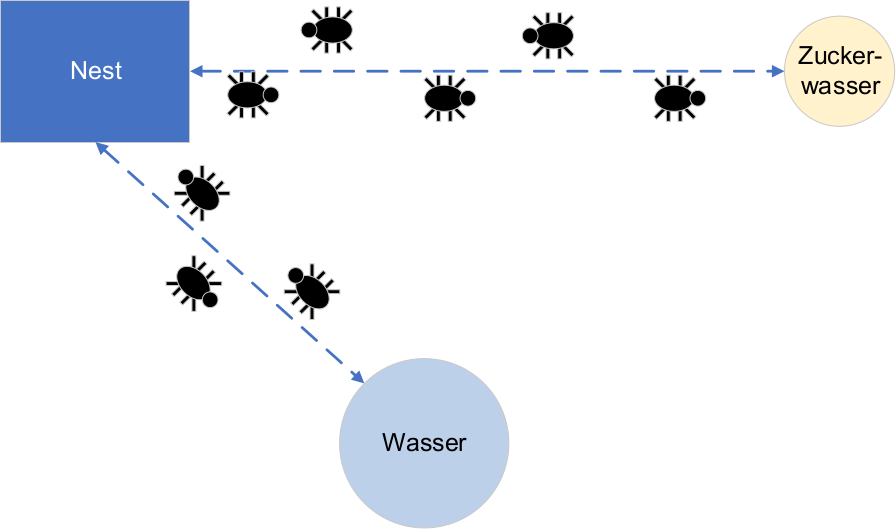
\includegraphics[width=0.7\linewidth]{images/AntAlgorithm_alphaEbeta.png}
		\caption{Modellierung der Parametereinstellung, sodass der Wert Alpha genauso groß ist wie der von Beta.}
		\label{parameter_a=b}
	\end{figure}
	Hier lässt sich die Aussage treffen, dass das Verhalten der neuen Ameisenkolonie aus Abbildung \ref{parameter_start} - sowie auch der späteren implementierten Software - diesem Zustand stark ähnelt. In beiden Fällen ist die Gewichtung ausgeglichen. Im Fall einer normalen Ameisenkolonie liegt dies aber an der noch nicht gewichteten Pheromonmatrix, die sich erst mit der Zeit aufbaut. 
	
	\subsection{$\alpha$ niedrig - $\beta$ hoch}
	Als letztes Beispiel - und auch letzten Abschnitt - folgt das Beispiel, dass die Länge der zu wählenden Strecke deutlich höher gewichtet ist als der Pheromonwert. Dies führt, wie in Abbildung \ref{parameter_a<b} zu sehen ist, dazu, dass nur einzelne Ameisen den Weg zum wertvolleren Zuckerwasser wählen. Denn die Strecke ist hierbei länger und somit weniger attraktiv.
	\begin{figure}[h]
		\centering
		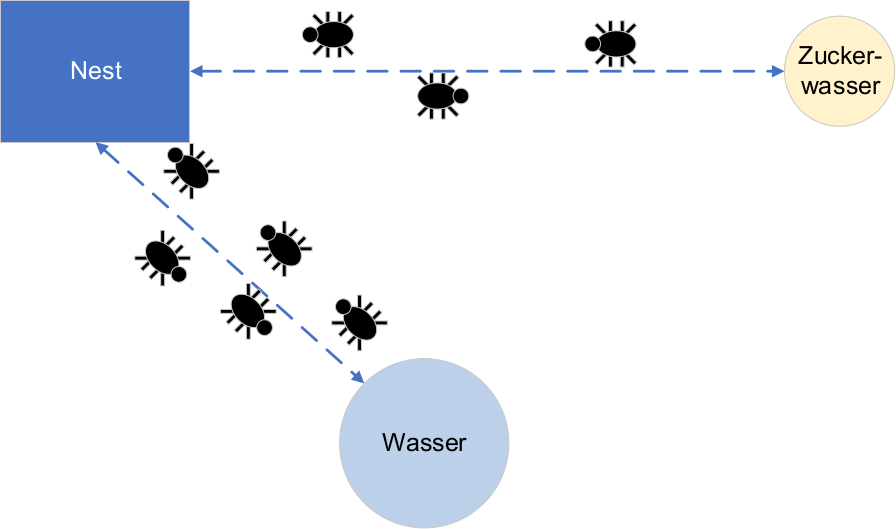
\includegraphics[width=0.7\linewidth]{images/AntAlgorithm_alphaLbeta.png}
		\caption{Modellierung der Parametereinstellung, sodass der Wert Alpha merklich kleiner als der von Beta ist.}
		\label{parameter_a<b}
	\end{figure}
	Dies hat wieder für die Ameisenkolonie eine allgemeine Folge, die sich auch auf die Software übertragen würde. Denn hier würde nur mit minimaler Wahrscheinlichkeit eine Verbesserung eintreten. Zum Einen weil die Pheromongewichtung auf dem besseren Pfad nie höher aufgebaut werden kann.\footnote{Hier sei noch erwähnt, dass alle Ameisen ihre Pheromone abgeben, sodass selbst die Ameisen auf dem Weg zum Wasser diesen Weg mit Pheromonen belegen. Dies hat den Effekt, dass durch die schiere Zahl an Ameisen dieser Weg einen höheren Pheromonwert besitzt.} Zum Anderen da eine Auswahl sowieso nur mit geringer Wahrscheinlichkeit zugunsten der Pheromonmatrix ausfallen würden.
}